% Created 2021-05-12 Wed 14:08
% Intended LaTeX compiler: pdflatex
\documentclass[11pt]{article}
\usepackage[utf8]{inputenc}
\usepackage[T1]{fontenc}
\usepackage{graphicx}
\usepackage{grffile}
\usepackage{longtable}
\usepackage{wrapfig}
\usepackage{rotating}
\usepackage[normalem]{ulem}
\usepackage{amsmath}
\usepackage{textcomp}
\usepackage{amssymb}
\usepackage{capt-of}
\usepackage{hyperref}
\usepackage[margin=0.5in]{geometry}
\usepackage{pgfplots}
\author{Hee Hwang and Sudarshan Raghavan}
\date{\today}
\title{Tasks}
\hypersetup{
 pdfauthor={Hee Hwang and Sudarshan Raghavan},
 pdftitle={Tasks},
 pdfkeywords={},
 pdfsubject={},
 pdfcreator={Emacs 26.3 (Org mode 9.1.9)}, 
 pdflang={English}}
\begin{document}

\maketitle






\section{Baseline}
\label{sec:org85b9722}
ACL  : Citation Intent Classification\\
Hyper: HyperPartisan News Detection\\
RCT  : Randomized Controlled Trials

\subsection{Baseline}
\label{sec:orgd55cbbc}
\begin{center}
\begin{tabular}{|c|c|c|c|c|}
\hline
Task & train & dev & test & Classes\\
\hline
ACL & 1688 & 114 & 139 & 6\\
\hline
Hyper & 516 & 64 & 65 & 2\\
\hline
RCT-sample & 500 & 30212 & 30135 & 5\\
\hline
RCT-200k & 180040 & 30212 & 30135 & 5\\
\hline
\end{tabular}
\end{center}




\section{Tables \& Plots}
\label{sec:orgf21a570}

\subsection{Augmentation by Distance}
\label{sec:org5891a92}
\subsubsection{Size Table}
\label{sec:org75617dd}
\begin{center}
\begin{tabular}{|c|c|c|c|}
\hline
Max Distance & ACL & Hyper & RCT\(_{\emph{sample}}\)\\
\hline
Baseline & 1688 (100\%) & 516 (100\%) & 500(100\%)\\
\hline
24 & 1746 (103\%) & 551 (106\%) & 686(137\%)\\
\hline
26 & 1815 (107\%) & 567 (109\%) & 831(166\%)\\
\hline
28 & 1981 (117\%) & 606 (117\%) & 1065(213\%)\\
\hline
30 & 2253 (133\%) & 656 (127\%) & 1484(296\%)\\
\hline
32 & 2842 (168\%) & 742 (143\%) & 2105(421\%)\\
\hline
34 & 3848 (227\%) & 911 (176\%) & 2952(590\%)\\
\hline
36 & 5819 (344\%) & 1127 (218\%) & 4196(839\%)\\
\hline
\end{tabular}
\end{center}
\subsubsection{Size Plot}
\label{sec:orgf821eb4}


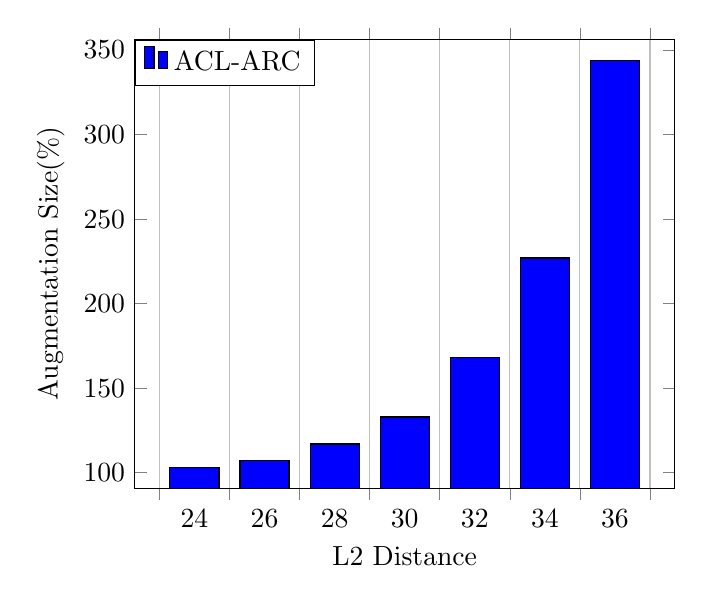
\begin{tikzpicture}
\begin{axis}[
	x tick label style={
		/pgf/number format/1000 sep=},
	xlabel=L2 Distance,
	ylabel=Augmentation Size(\%),
	enlargelimits=0.05,
	ybar interval=0.7,
  legend style={at={(0,1)},anchor=north west}
]
\addplot[fill=blue] 
	coordinates {(24,103) (26,107) (28,117) (30,133) (32,168) (34,227) (36,344) (38,344)};
\addlegendentry{ACL-ARC}
\end{axis}
\end{tikzpicture}

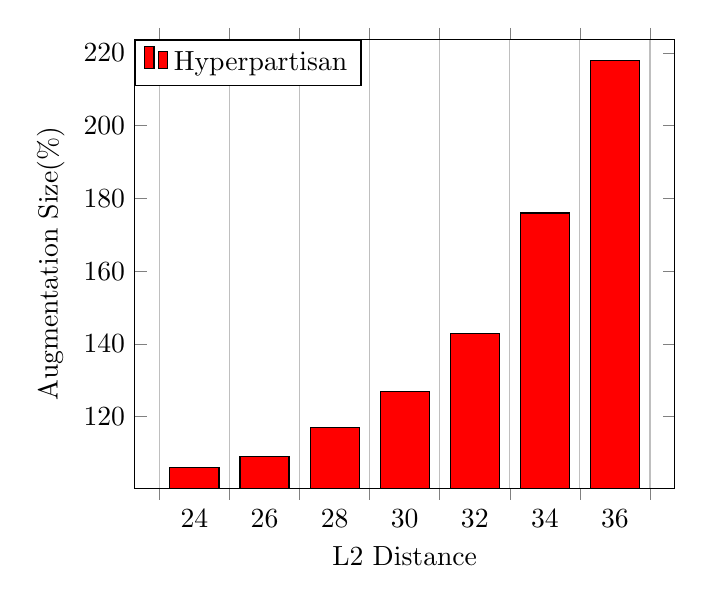
\begin{tikzpicture}
\begin{axis}[
	x tick label style={
		/pgf/number format/1000 sep=},
	xlabel=L2 Distance,
	ylabel=Augmentation Size(\%),
	enlargelimits=0.05,
	ybar interval=0.7,
  legend style={at={(0,1)},anchor=north west}
]
\addplot[fill=red]
	coordinates {(24,106) (26,109) (28,117) (30,127) (32,143) (34,176) (36,218) (38,218)};
\addlegendentry{Hyperpartisan}
\end{axis}
\end{tikzpicture}


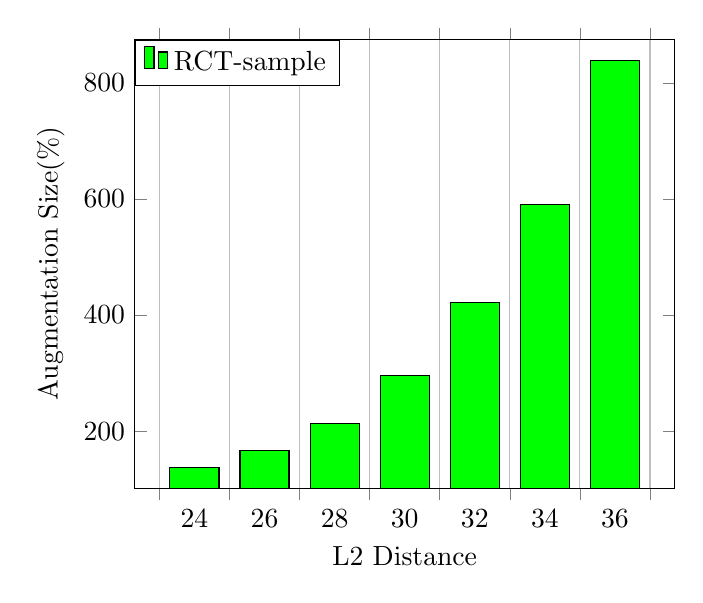
\begin{tikzpicture}
\begin{axis}[
	x tick label style={
		/pgf/number format/1000 sep=},
	xlabel=L2 Distance,
	ylabel=Augmentation Size(\%),
	enlargelimits=0.05,
	ybar interval=0.7,
  legend style={at={(0,1)},anchor=north west}
]
\addplot[fill=green]
	coordinates {(24,137) (26,166) (28,213) (30,296) (32,421) (34,590) (36,839) (38,839)};
\addlegendentry{RCT-sample}
\end{axis}
\end{tikzpicture}







\subsubsection{F1 Table}
\label{sec:org47718b9}
\begin{center}
\begin{tabular}{|c|c|c|c|}
\hline
Max Distance & ACL & Hyper & RCT\(_{\emph{sample}}\)\\
\hline
Baseline & 62.70 & 90.24 & 73.60\\
\hline
24 & 65.77(\textpm{} 7.40) & 92.68(\textpm{} 3.29) & 69.33(\textpm{} 0.73)\\
\hline
26 & 66.79(\textpm{} 3.07) & 90.63(\textpm{} 5.92) & 67.31(\textpm{} 1.96)\\
\hline
28 & 63.93(\textpm{} 3.67) & 92.66(\textpm{} 4.39) & 63.91(\textpm{} 1.25)\\
\hline
30 & 62.57(\textpm{} 2.70) & 89.60(\textpm{} 5.04) & 60.43(\textpm{} 0.64)\\
\hline
32 & 64.83(\textpm{} 5.28) & 90.15(\textpm{} 5.22) & 57.23(\textpm{} 1.27)\\
\hline
34 & 57.06(\textpm{} 3.05) & 88.36(\textpm{} 3.26) & 54.36(\textpm{} 1.31)\\
\hline
36 & 56.20(\textpm{} 4.21) & 89.49(\textpm{} 2.40) & 52.76(\textpm{} 0.85)\\
\hline
\end{tabular}
\end{center}

\subsubsection{F1 Plot}
\label{sec:orgeaeb413}
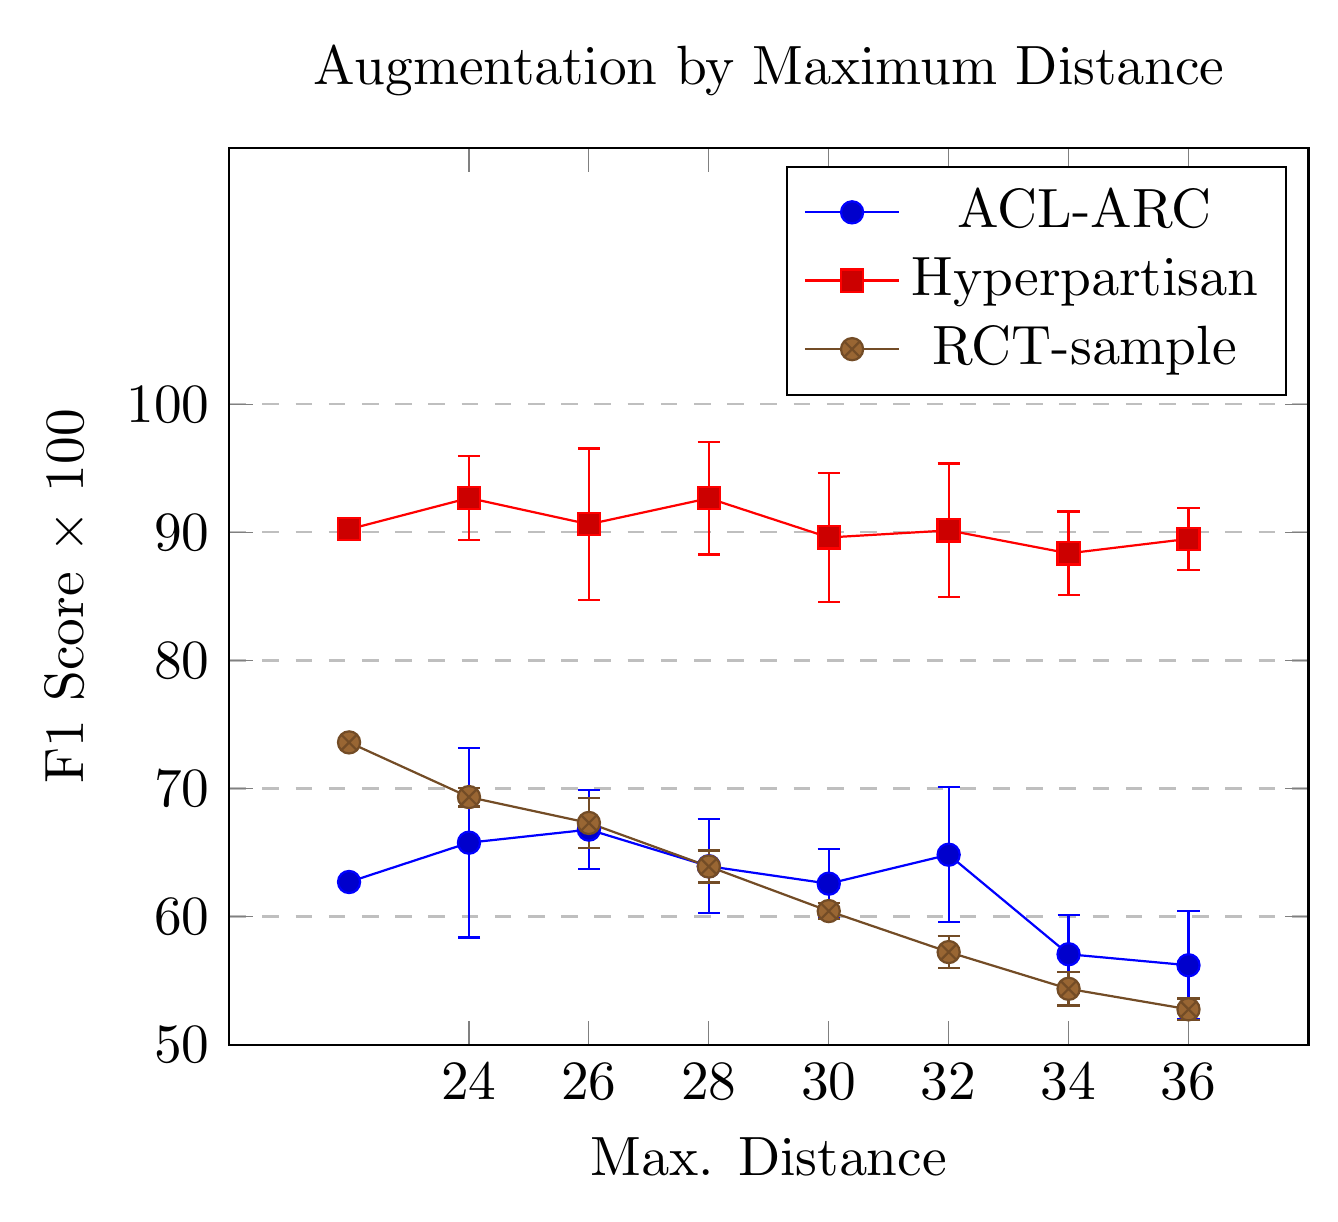
\begin{tikzpicture}[thick,scale=2.0]
\begin{axis}[
    title={Augmentation by Maximum Distance},
    xlabel={Max. Distance},
    ylabel={F1 Score $\times$ 100},
    xmin=20, xmax=38,
           ymin=50, ymax=120,
    xtick={24,26,28,30,32,34,36},
    ytick={50,60,70,80,90,100},
    ymajorgrids=true,
    grid style=dashed,       
]
\addplot+ [error bars/.cd, y dir=both, y explicit,]
    coordinates {
    (22,62.70)
    (24,65.77) +- (0,7.40)
    (26,66.79) +- (0,3.07)
    (28,63.93) +- (0,3.67) 
    (30,62.57) +- (0,2.70)
    (32,64.83) +- (0,5.28)
    (34,57.06) +- (0,3.05)
    (36,56.20) +- (0,4.21)
    };
    \addlegendentry{ACL-ARC}
\addplot+ [error bars/.cd, y dir=both, y explicit,]
    coordinates {
    (22,90.24)
    (24,92.68) +- (0,3.29)
    (26,90.63) +- (0,5.92)
    (28,92.66) +- (0,4.39)
    (30,89.60) +- (0,5.04)
    (32,90.15) +- (0,5.22)
    (34,88.36) +- (0,3.26)
    (36,89.49) +- (0,2.40)
    };
    \addlegendentry{Hyperpartisan}
\addplot+ [error bars/.cd, y dir=both, y explicit,]
    coordinates {
    (22,73.60)
    (24,69.33) +- (0,0.73)
    (26,67.31) +- (0,1.96)
    (28,63.91) +- (0,1.25)
    (30,60.43) +- (0,0.64)
    (32,57.23) +- (0,1.27)
    (34,54.36) +- (0,1.31)
    (36,52.76) +- (0,0.85)
    };
    \addlegendentry{RCT-sample}
\end{axis}
\end{tikzpicture}


\subsection{Augmentation by Fixed Size}
\label{sec:org47655dc}
\subsubsection{F1 Table}
\label{sec:orgb98bf1e}
\begin{center}
\begin{tabular}{|c|c|c|c|c|}
\hline
Aug Data & ACL & Hyper & RCT\(_{\emph{sample}}\)\\
\hline
Baseline & 62.70 & 90.24 & 73.60\\
\hline
1 & 65.28(\textpm{} 5.05) & 89.12(\textpm{} 7.31) & 71.65(\textpm{} 1.97)\\
\hline
2 & 64.71(\textpm{} 3.61) & 90.74(\textpm{} 3.94) & 71.20(\textpm{} 0.99)\\
\hline
3 & 66.73(\textpm{} 3.72) & 90.94(\textpm{} 4.54) & 72.04(\textpm{} 0.20)\\
\hline
4 & 65.26(\textpm{} 3.20) & 92.64(\textpm{} 4.59) & 72.27(\textpm{} 1.31)\\
\hline
5 & 65.80(\textpm{} 3.10) & 93.28(\textpm{} 2.62) & 71.68(\textpm{} 0.71)\\
\hline
6 & 65.39(\textpm{} 4.23) & 89.11(\textpm{} 5.22) & 71.96(\textpm{} 0.87)\\
\hline
7 & 63.25(\textpm{} 2.51) & 89.90(\textpm{} 4.97) & 71.78(\textpm{} 1.07)\\
\hline
8 & 65.81(\textpm{} 2.13) & 87.84(\textpm{} 6.20) & 71.75(\textpm{} 0.66)\\
\hline
9 & 66.85(\textpm{} 6.14) & 91.23(\textpm{} 2.50) & 71.77(\textpm{} 0.97)\\
\hline
10 & 62.68(\textpm{} 3.29) & 91.54(\textpm{} 4.01) & 71.32(\textpm{} 0.54)\\
\hline
\end{tabular}
\end{center}

\subsubsection{F1 Plot}
\label{sec:org8ae0013}
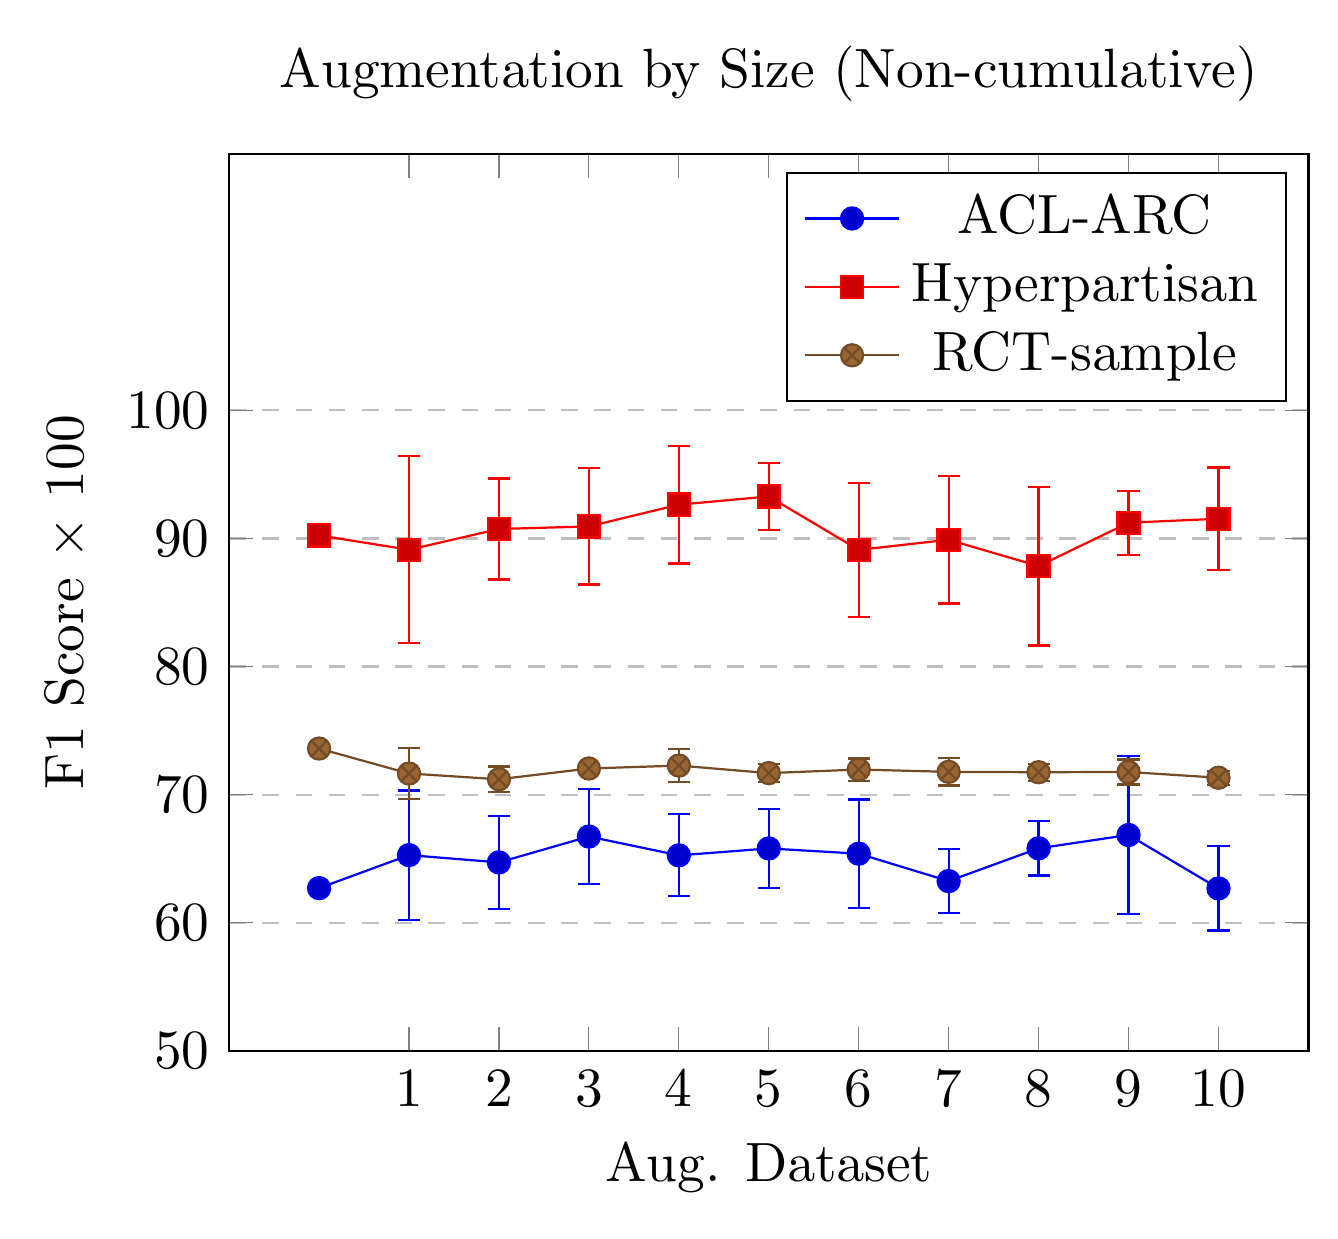
\begin{tikzpicture}[thick,scale=2.0]
\begin{axis}[
    title={Augmentation by Size (Non-cumulative)},
    xlabel={Aug. Dataset},
    ylabel={F1 Score $\times$ 100},
    xmin=-1, xmax=11,
    ymin=50, ymax=120,
    xtick={1,2,3,4,5,6,7,8,9,10},
    ytick={50,60,70,80,90,100},
    ymajorgrids=true,
    grid style=dashed,
]

\addplot+ [error bars/.cd, y dir=both, y explicit,]
    coordinates {
    (0,62.70)
    (1,65.28)  +- (0,5.05)
    (2,64.71)  +- (0,3.61)
    (3,66.73)  +- (0,3.72)
    (4,65.26)  +- (0,3.20)
    (5,65.80)  +- (0,3.10)
    (6,65.39)  +- (0,4.23)
    (7,63.25)  +- (0,2.51)
    (8,65.81)  +- (0,2.13)
    (9,66.85)  +- (0,6.14)
    (10,62.68) +- (0,3.29)
    };
    \addlegendentry{ACL-ARC}

\addplot+ [error bars/.cd, y dir=both, y explicit,]
     coordinates {
     (0,90.24)
     (1,89.12)  +- (0,7.31)
     (2,90.74)  +- (0,3.94)
     (3,90.94)  +- (0,4.54)
     (4,92.64)  +- (0,4.59)
     (5,93.28)  +- (0,2.62)
     (6,89.11)  +- (0,5.22)
     (7,89.90)  +- (0,4.97)
     (8,87.84)  +- (0,6.20)
     (9,91.23)  +- (0,2.50)
     (10,91.54) +- (0,4.01)
     };
     \addlegendentry{Hyperpartisan}

\addplot+ [error bars/.cd, y dir=both, y explicit,]
     coordinates {
     (0,73.60)   
     (1,71.65)  +- (0,1.97)
     (2,71.20)  +- (0,0.99)
     (3,72.04)  +- (0,0.20)
     (4,72.27)  +- (0,1.31) 
     (5,71.68)  +- (0,0.71)
     (6,71.96)  +- (0,0.87)
     (7,71.78)  +- (0,1.07)
     (8,71.75)  +- (0,0.66)
     (9,71.77)  +- (0,0.97)
     (10,71.32) +- (0,0.54)
     };
     \addlegendentry{RCT-sample}

\end{axis}
\end{tikzpicture}



\section{Baseline models:}
\label{sec:org6a8d233}
\begin{itemize}
\item An off-the-shelf RoBERTa model that has been finetuned to perform classification for each of the downstream tasks
\end{itemize}

\section{Augmentation Model}
\label{sec:org2d61b07}
\begin{center}
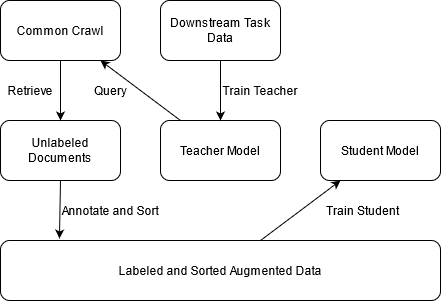
\includegraphics[width=.9\linewidth]{./png/da.png}
\end{center}


\section{Algorithm}
\label{sec:org51e74ee}
\begin{verbatim}
1. Extract failed test examples from the baseline model
2. Retrieve passages/sentences from Common Crawl 
3. Apply augmentation strategy (i)-(iii)
4. Augment all the labelled CC data to the training data
5. Retrain RoBERTa on the augmented training set 
\end{verbatim}

\section{Augmentation Strategies}
\label{sec:org59de0c0}
\begin{itemize}
\item Strategy (i)\\
Use baseline model (Teacher) to perform unsupervised labelling on retrieved CC data
\item Strategy (ii)\\
Using a task specific binary classifier, 
filter out retrieved CC data that is "out-domain"\\
Use baseline model (Teacher) to perform unsupervised labelling on the filtered "in-domain" CC data
\item Strategy (iii)\\
Using a task specific binary classifier, 
filter out retrieved CC data that is "out-domain"\\
Use ground truth labels of failed test examples and assign labels to the filtered "in-domain" CC data
\end{itemize}
\end{document}
